\documentclass[tikz,border=6pt]{standalone}
\usepackage[T1]{fontenc}
\usepackage{newtxtext,newtxmath}
\usepackage{tikz}
\usetikzlibrary{arrows.meta,positioning,calc,backgrounds}

\definecolor{ink}{HTML}{172033}
\definecolor{greyLine}{HTML}{9CA3AF}
\definecolor{greyFill}{HTML}{F3F4F6}
\definecolor{qkC}{HTML}{B91C1C}
\definecolor{ovC}{HTML}{0B7285}
\definecolor{steerC}{HTML}{2E7D32}

\tikzset{
  >={Latex[length=2.4mm,width=1.7mm]},
  ctitle/.style={font=\bfseries,text=ink,align=center},
  note/.style={font=\scriptsize,text=steerC,align=center},
  rowlab/.style={font=\small\bfseries,align=center},
  poslab/.style={font=\scriptsize\bfseries,text=ink,align=center},
  feat/.style={draw,line width=0.8pt,rounded corners=2pt,minimum width=10mm,
    minimum height=8.5mm,font=\small\bfseries,text=ink,inner sep=1pt,fill=white},
  knob/.style={circle,draw=steerC,fill=steerC,text=white,font=\tiny\bfseries,
    inner sep=0.3pt,minimum size=4mm,line width=0.4pt},
  keytxt/.style={font=\scriptsize,text=ink,align=left,anchor=west},
}
% \gauge{x}{y}{act in [-1,1]}{fillcolor}
\newcommand{\gauge}[4]{%
  \draw[greyLine,line width=0.4pt,fill=white] (#1-1.2,#2-5.5) rectangle (#1+1.2,#2+5.5);
  \fill[#4] (#1-1.2,#2) rectangle (#1+1.2,#2+#3*5);
  \draw[greyLine,line width=0.5pt] (#1-1.2,#2) -- (#1+1.2,#2);
}

\begin{document}
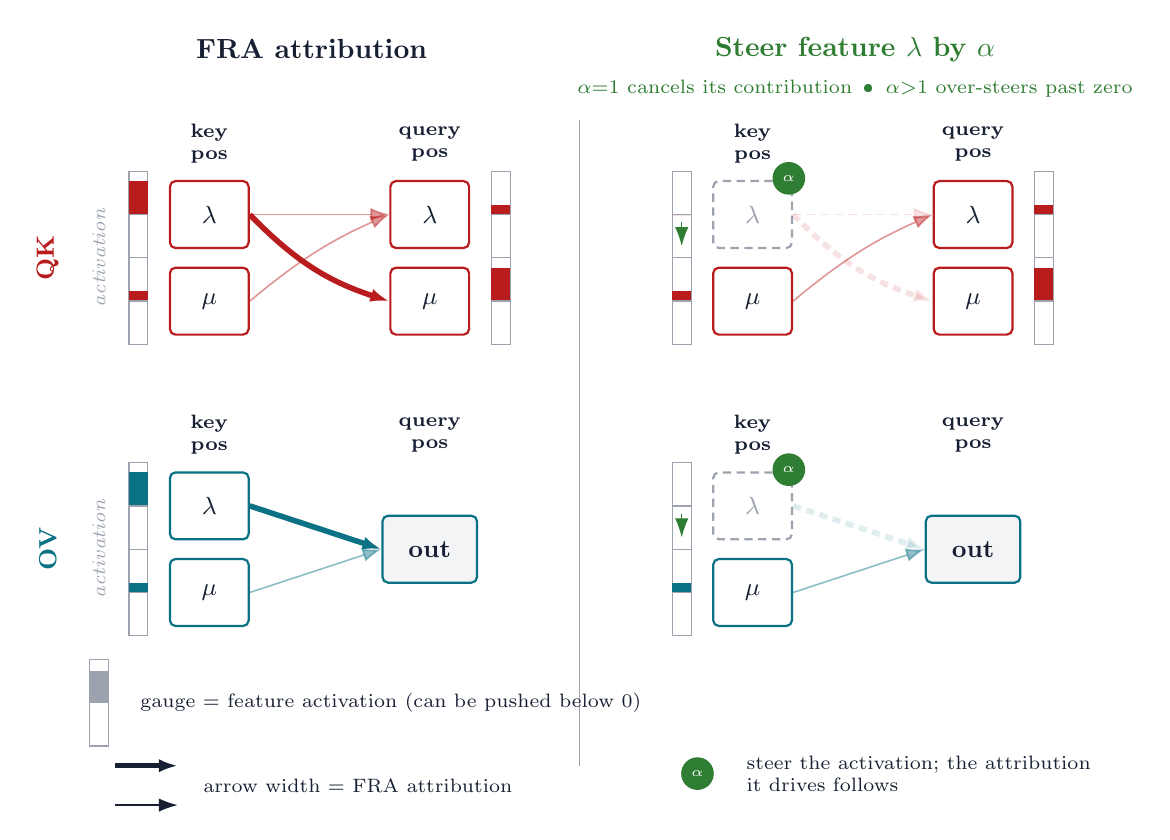
\begin{tikzpicture}[x=1mm,y=1mm]

\node[ctitle] at (35,95) {FRA attribution};
\node[ctitle,text=steerC] at (104,95) {Steer feature $\lambda$ by $\alpha$};
\node[note] at (104,90) {$\alpha{=}1$ cancels its contribution \,\textbullet\, $\alpha{>}1$ over-steers past zero};
\draw[greyLine,line width=0.4pt] (69,4) -- (69,86);

\node[rowlab,text=qkC,rotate=90] at (1.5,68.5) {QK};
\node[rowlab,text=ovC,rotate=90] at (1.5,31.5) {OV};
\node[font=\scriptsize\itshape,text=greyLine,rotate=90] at (8,68.5) {activation};
\node[font=\scriptsize\itshape,text=greyLine,rotate=90] at (8,31.5) {activation};

% ================= LEFT COLUMN =================
\node[poslab] at (22,83) {key\\pos}; \node[poslab] at (50,83) {query\\pos};
\gauge{13}{74}{0.85}{qkC} \node[feat,draw=qkC] (Lk1) at (22,74) {$\lambda$};
\gauge{13}{63}{0.25}{qkC} \node[feat,draw=qkC] (Lk2) at (22,63) {$\mu$};
\gauge{59}{74}{0.25}{qkC} \node[feat,draw=qkC] (Lq1) at (50,74) {$\lambda$};
\gauge{59}{63}{0.85}{qkC} \node[feat,draw=qkC] (Lq2) at (50,63) {$\mu$};
\draw[->,qkC,line width=0.6pt,opacity=0.45] (Lk1.east) -- (Lq1.west);
\draw[->,qkC,line width=0.6pt,opacity=0.45] (Lk2.east) to[bend left=8] (Lq1.west);
\draw[->,qkC,line width=2.0pt] (Lk1.east) to[bend right=14] (Lq2.west);
\node[poslab] at (22,46) {key\\pos}; \node[poslab] at (50,46) {query\\pos};
\gauge{13}{37}{0.85}{ovC} \node[feat,draw=ovC] (Lo1) at (22,37) {$\lambda$};
\gauge{13}{26}{0.25}{ovC} \node[feat,draw=ovC] (Lo2) at (22,26) {$\mu$};
\node[feat,draw=ovC,fill=greyFill,minimum width=12mm] (Lout) at (50,31.5) {out};
\draw[->,ovC,line width=2.0pt] (Lo1.east) -- (Lout.west);
\draw[->,ovC,line width=0.6pt,opacity=0.45] (Lo2.east) -- (Lout.west);

% ================= RIGHT COLUMN (steer lambda to ~0, hint beyond) =================
\node[poslab] at (91,83) {key\\pos}; \node[poslab] at (119,83) {query\\pos};
\gauge{82}{74}{0.0}{qkC} \draw[steerC,line width=0.5pt,->,densely dashed] (82,73) -- (82,70);
\node[feat,draw=greyLine,densely dashed,text=greyLine] (Rk1) at (91,74) {$\lambda$};
\node[knob] at ([xshift=4.6mm,yshift=4.6mm]Rk1.center) {$\alpha$};
\gauge{82}{63}{0.25}{qkC} \node[feat,draw=qkC] (Rk2) at (91,63) {$\mu$};
\gauge{128}{74}{0.25}{qkC} \node[feat,draw=qkC] (Rq1) at (119,74) {$\lambda$};
\gauge{128}{63}{0.85}{qkC} \node[feat,draw=qkC] (Rq2) at (119,63) {$\mu$};
\draw[->,qkC,line width=0.6pt,densely dashed,opacity=0.13] (Rk1.east) -- (Rq1.west);
\draw[->,qkC,line width=0.6pt,opacity=0.45] (Rk2.east) to[bend left=8] (Rq1.west);
\draw[->,qkC,line width=2.0pt,densely dashed,opacity=0.13] (Rk1.east) to[bend right=14] (Rq2.west);
\node[poslab] at (91,46) {key\\pos}; \node[poslab] at (119,46) {query\\pos};
\gauge{82}{37}{0.0}{ovC} \draw[steerC,line width=0.5pt,->,densely dashed] (82,36) -- (82,33);
\node[feat,draw=greyLine,densely dashed,text=greyLine] (Ro1) at (91,37) {$\lambda$};
\node[knob] at ([xshift=4.6mm,yshift=4.6mm]Ro1.center) {$\alpha$};
\gauge{82}{26}{0.25}{ovC} \node[feat,draw=ovC] (Ro2) at (91,26) {$\mu$};
\node[feat,draw=ovC,fill=greyFill,minimum width=12mm] (Rout) at (119,31.5) {out};
\draw[->,ovC,line width=2.0pt,densely dashed,opacity=0.13] (Ro1.east) -- (Rout.west);
\draw[->,ovC,line width=0.6pt,opacity=0.45] (Ro2.east) -- (Rout.west);

% ================= LEGEND =================
\gauge{8}{12}{0.8}{greyLine}
\node[keytxt] at (12,12) {gauge $=$ feature activation (can be pushed below $0$)};
\draw[->,ink,line width=2.0pt] (10,4) -- (18,4);
\draw[->,ink,line width=0.6pt] (10,-1) -- (18,-1);
\node[keytxt] at (20,1.5) {arrow width $=$ FRA attribution};
\node[knob] at (84,3) {$\alpha$};
\node[keytxt,text width=44mm] at (89,3) {steer the activation; the attribution it drives follows};

\end{tikzpicture}
\end{document}
